\documentclass[11pt,a4paper,oneside]{report}

\usepackage{pdfpages}
\usepackage{epstopdf}
\usepackage{url}
\usepackage{subfig}
\usepackage[toc,page]{appendix}
\usepackage{hyperref}



\renewcommand{\thesection}{\arabic{section}}
\setcounter{secnumdepth}{3}

\title{\textbf{Master thesis : Fake news detection using machine learning}
\\ Review 1}

\author{Simon Lorent}

\date{Academic year 2018 - 2019}

\begin{document}
\maketitle
\section{Data}
\subsection{Sources}
\paragraph{} The data is comming from \href{https://github.com/several27/FakeNewsCorpus}{Fake News Corpus} which compiles news from different sources that have been built according to \href{http://www.opensources.co/}{OpenSources} initiative. It is made of around 9.5 millions news, classified in 11 categories. A second data set is used as a test set and is comming from \href{https://github.com/KaiDMML/FakeNewsNet}{FakeNewsNet} and is quite smaller. 

\subsection{Preliminary data exploration}
\paragraph{} In order to have some insight of the first data set, some statistical exploration have been made. The first thing that have been made is data cleaning, as it comes as a 30GB csv file, loading the complete file in momery is not possible. In order to overcome this difficulty, mongodb have been used. As the csv file is not entierly formated correclty, badly formated lines are thrown away. After this very early cleaning, it lefts exaclty $8.125.732$ news in the database distributed as follows (see \textbf{figure \ref{plot:plot1}}):
\vspace{1em}
\begin{figure}[h]
	\centering
	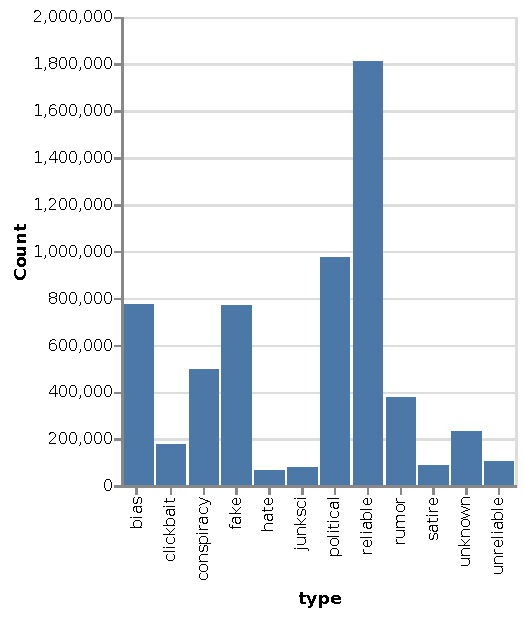
\includegraphics[width=0.5\textwidth]{plot1.pdf}
	\caption{Distrubtion of news by type. }
	\label{plot:plot1}
\end{figure}
Currently, only fake news and reliable news have been used. 

\paragraph{} Some statistics such as the number of sentences in the news and the average number of words per sentence have been computed and gave the follow result:
\begin{figure}[h]
	\centering
	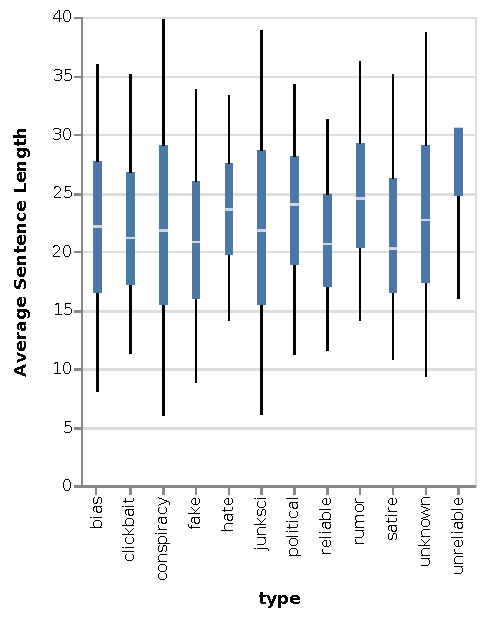
\includegraphics[width=0.5\textwidth]{plot2.pdf}
	\caption{Average number of words per sentences.}
	\label{plot:plot2}
\end{figure}
\begin{figure}[h]
	\centering
	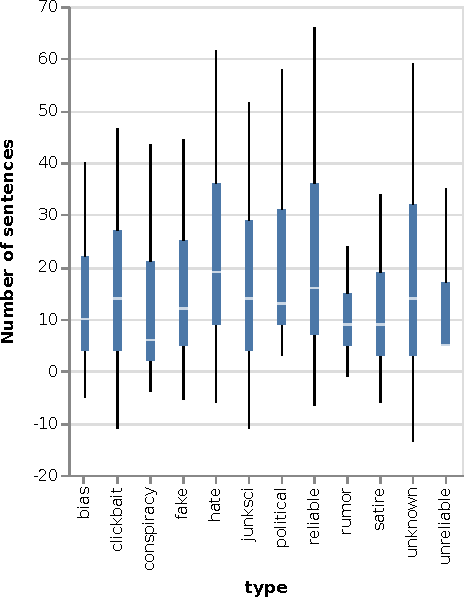
\includegraphics[width=0.5\textwidth]{plot3.pdf}
	\caption{Number of sentences}
	\label{plot:plot3}
\end{figure}
\paragraph{}
Outliers have been removed from the boxplot because some text formating prevent conting these quantities correctly. 

\section{First Model : Naive-Bayes}
\paragraph{} This model uses sklearn vectorizer in order to preprocess texts. Using k-folds cross validation, the vectorizer is fitted on the train data, and test data is simply transformed by the vectorizer. The model give accuracy : $0.8921$, $0.8924$, $0.8922$ for an average accuracy of $0.8981$ on the train data and $0.8923$ on test data. Training the model on the complete corpus and testing it on the second data set give the following results: 
\begin{table}[h]
\centering
\begin{tabular}{|l|l|l|l|}
\hline
 type & precision & recall & f1-score \\
 \hline
 fake & $0.752$ &  $0.33$ & $0.46$   \\
 reliable & $0.5714$  &  $0.890$ &  $0.696$ \\
 \hline
\end{tabular}
\end{table}
Which is not bad for a simple method. 

\section{Bias in the data set}
\paragraph{} After trying to explain the reason behind the results on the test set, it appears that the data set in biased. Indeed, must of the news came from the same sources. For instance, fake news moslty comes from \textit{beforeitsnews.com} and reliable news comes from \textit{nytimes.com}.
\begin{figure}[h]
	\centering
	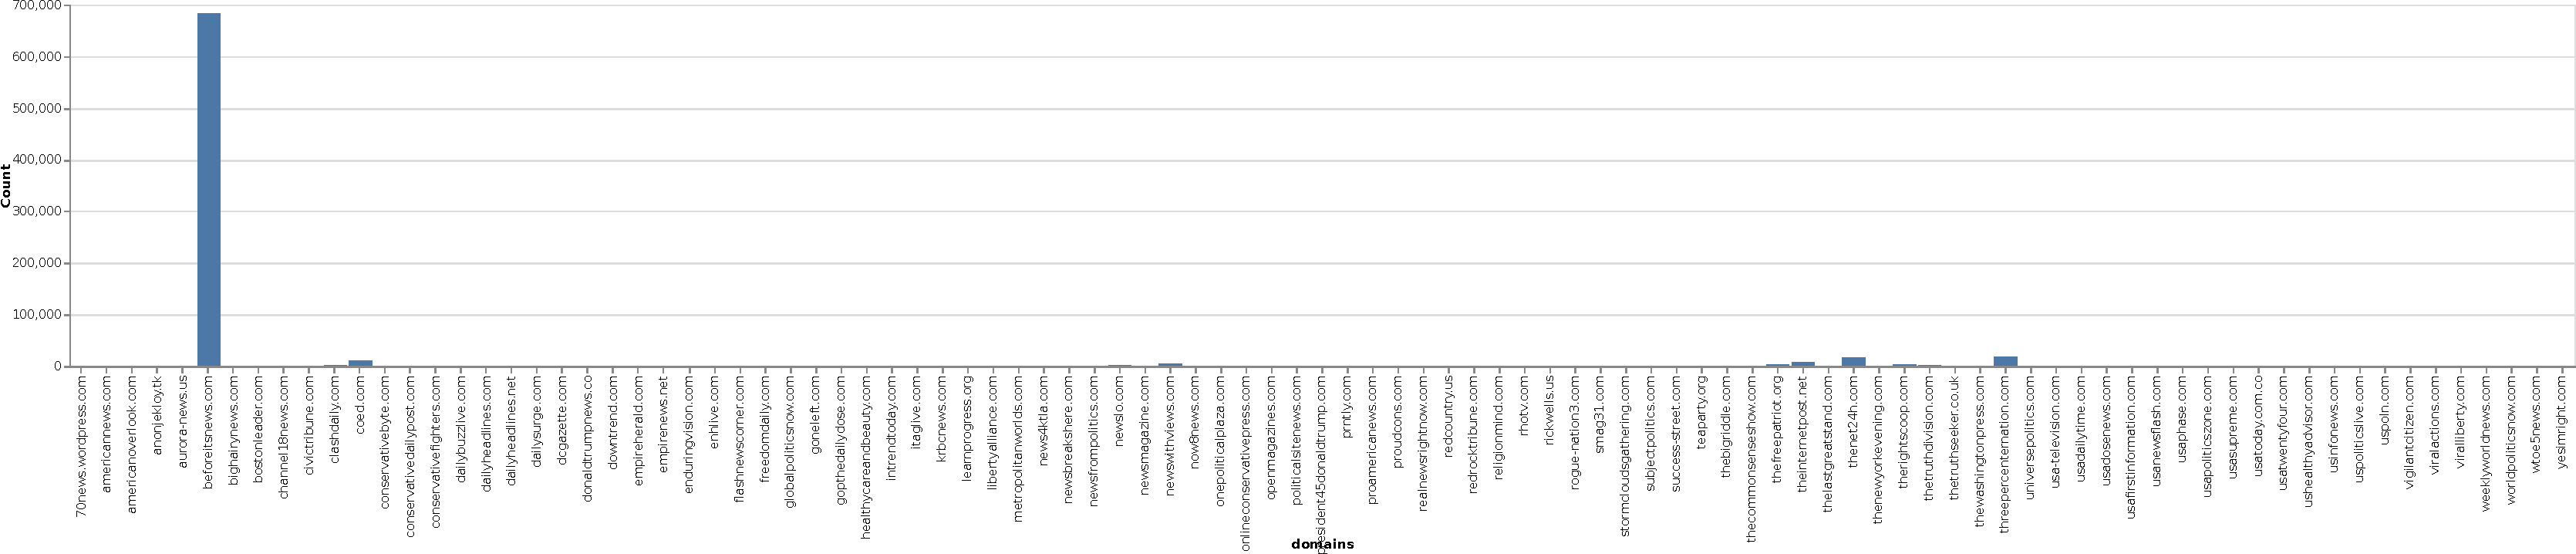
\includegraphics[width=1\textwidth]{fake.pdf}
	\caption{Fake news sources}
\end{figure}
\begin{figure}[h]
	\centering
	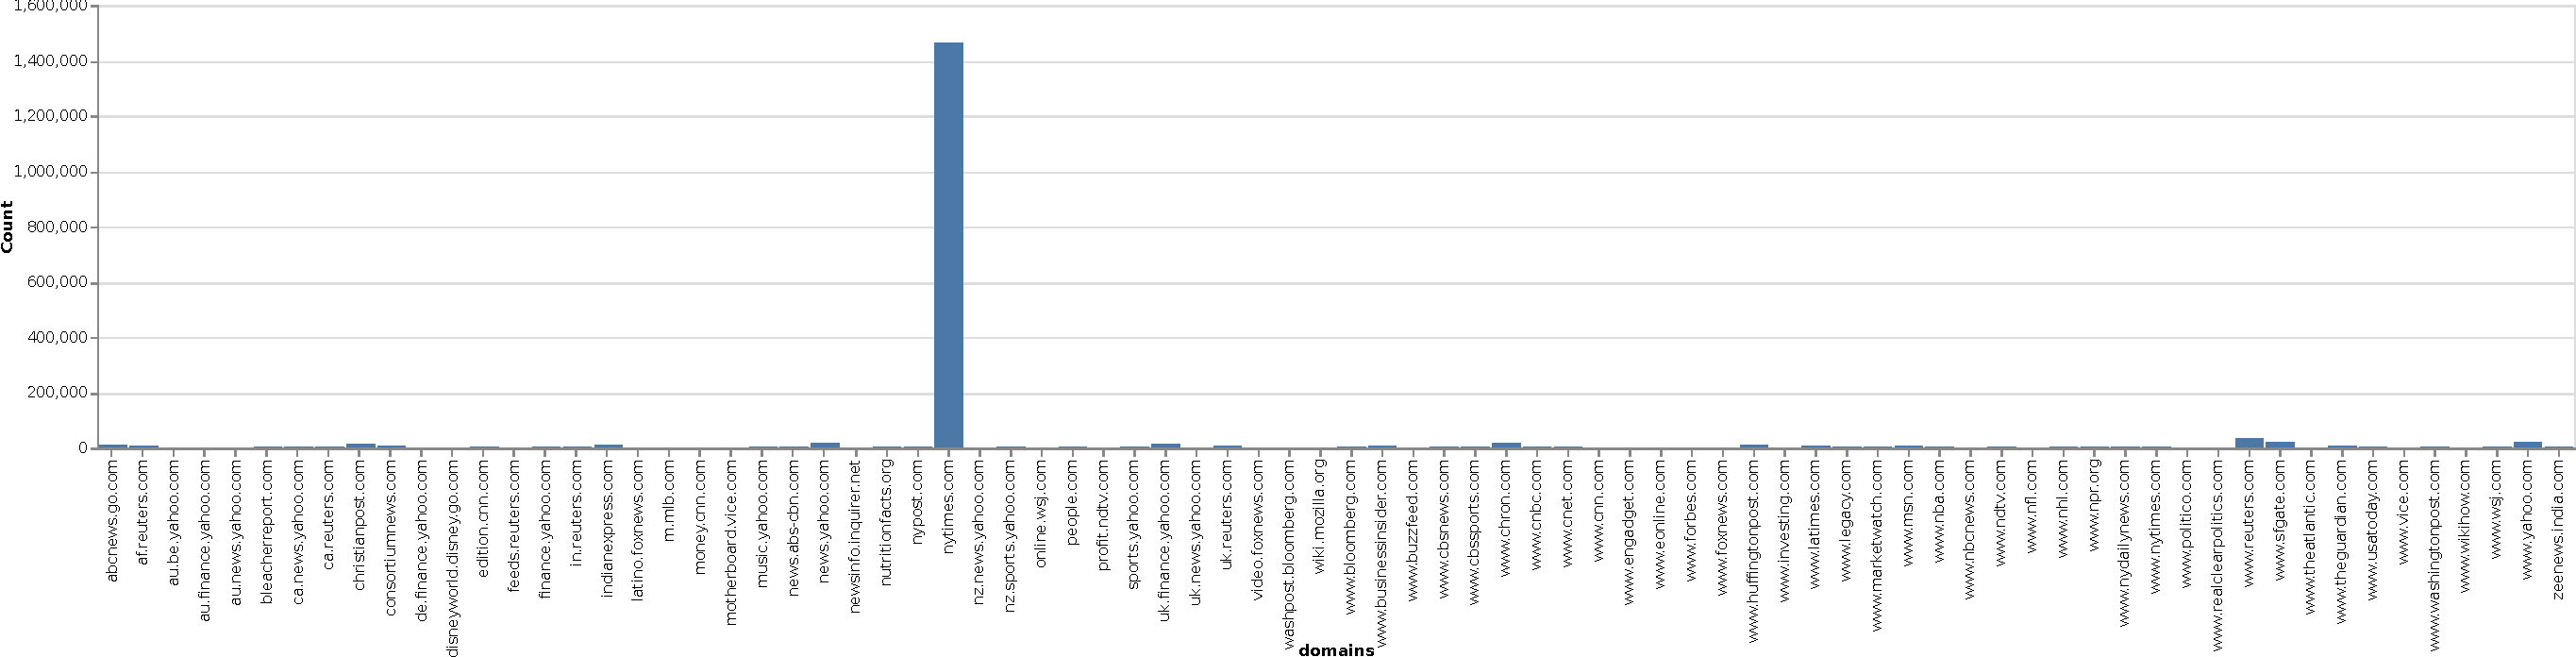
\includegraphics[width=1\textwidth]{reliable.pdf}
	\caption{Reliable news sources}
\end{figure}

This bias need to be overcome.

\section{Next objectives}
\begin{itemize}
	\item Word embedding using word2vec
	\item Making models on this embedding (Neural Networks, CNN, LSTM)
	\item Implementing C-LSTM \cite{Zhou2015}
\end{itemize}

\bibliographystyle{plain}
\bibliography{../references/references.bib}
\end{document}